\documentclass[12pt]{article}

\usepackage[utf8]{inputenc}
\usepackage[T1]{fontenc}
\usepackage[margin=1in]{geometry}
\usepackage{setspace}
\usepackage{amsmath, amssymb}
\usepackage{lmodern}
\usepackage{algorithm}
\usepackage{algpseudocode}
\usepackage{booktabs}
\usepackage{tikz}
\usepackage{float}
\usepackage{graphicx}
\usepackage{pgfgantt}
\usepackage{caption}
\usepackage{subcaption}
\usepackage{siunitx}
\usepackage{pgfplotstable}
\usepackage{multirow}
\usepackage[hidelinks]{hyperref}

\setstretch{1.2}
\setkeys{Gin}{draft=false}
\sisetup{round-mode=places,round-precision=2}

\pgfplotstableset{
  col sep=comma,
  every head row/.style={before row=\toprule,after row=\midrule},
  every last row/.style={after row=\bottomrule}
}

\begin{document}

% Custom title page
\begin{titlepage}
\centering

\vspace*{2cm}

% Institution at top
{\large Hacettepe University}

\vspace{2cm}

% Top horizontal rule
{\noindent\rule{\textwidth}{2pt}}

\vspace{1cm}

% Title
{\Huge\bfseries Time-Windowed Vehicle Routing Without Capacity Constraints:\\
\vspace{0.5cm}
A Dual-Pipeline Heuristic Framework}

\vspace{0.5cm}

{\Large\bfseries Project Final Report}\\
\vspace{0.3cm}
{\Large\bfseries EMU654 Heuristic Methods for Optimization}

\vspace{0.5cm}

% Bottom horizontal rule
{\noindent\rule{\textwidth}{2pt}}

\vfill

% Student information
{\large Student -- Mert Karaaslan}

\vspace{2cm}

% Date at bottom
{\large January 7, 2026}

\vspace{1cm}

\end{titlepage}

\newpage

% Table of Contents
\tableofcontents

\newpage

\begin{abstract}
This paper considers a variant of the Vehicle Routing Problem with Time Windows (VRPTW) in which vehicle capacity constraints are intentionally omitted in order to isolate time-related effects. Classical VRPTW models are primarily designed for freight settings where vehicle load limits are critical. By contrast, many contemporary service environments---such as field maintenance, technical support, or modular delivery systems---can flexibly adjust capacity, making temporal feasibility the main planning concern.

We develop a heuristic framework for this \emph{capacity-free} VRPTW that combines two classical construction heuristics, Nearest Neighbor and Clarke--Wright Savings, with a common sequence of local search operators (2-opt and relocation). The framework is organized as a dual-pipeline architecture: each pipeline constructs an initial solution using a different heuristic and then applies the same improvement procedures, after which the better solution is selected. This design enables a structured comparison of construction strategies under identical local search conditions and provides a clean setting for analyzing how time-window interactions alone shape route structure. The proposed methodology is intended as a baseline heuristic framework for time-dominant routing problems and as a starting point for future empirical studies in capacity-free VRPTW.
\end{abstract}

\noindent\textbf{Keywords:} Vehicle Routing Problem, Time Windows, Heuristics, Local Search, Nearest Neighbor, Clarke--Wright, Temporal Optimization, Service Operations.

\section{Introduction}

\subsection{Background and Motivation}

The Vehicle Routing Problem (VRP) is a central topic in operations research and combinatorial optimization, addressing the design of efficient routes from a depot to a set of geographically distributed customers. Since the seminal study of Dantzig and Ramser (1959), the VRP family has expanded to include many practical features, such as capacity limitations, time windows, multiple depots, pickup-and-delivery requirements, and periodic planning structures. Within this family, the Vehicle Routing Problem with Time Windows (VRPTW) is particularly relevant for modern service and distribution systems, where satisfying customer-specific service intervals is as important as minimizing travel distance. In VRPTW, each customer must be served within a specified time window $[a_i, b_i]$, which constrains feasible visit sequences and introduces substantial temporal complexity. The problem is NP-hard, and time windows make the problem even harder by restricting admissible service orders.

Most classical VRPTW formulations assume fixed and binding vehicle capacities. This assumption is appropriate for freight-oriented operations, such as bulk distribution or fuel transportation, where load feasibility strongly drives route design. However, many contemporary service and urban logistics applications exhibit flexible or dynamically adjustable capacity. Examples include field-service teams, on-demand maintenance crews, medical response units, and modular delivery systems, where vehicle size or the number of service teams can be chosen after routes are planned or adjusted in response to workload. In such environments, route feasibility is driven less by vehicle load and more by the interplay of time-window adherence, service durations, and travel times.

Motivated by these applications, this study focuses on a \emph{capacity-free} variant of VRPTW. Load constraints are removed explicitly so that the core temporal optimization problem can be examined in isolation: sequences of customers must be chosen such that all time windows are satisfied and total travel distance (or time) is minimized. This perspective serves two main purposes. First, it clarifies how time-window constraints alone shape route structure, including the propagation of early or late arrivals, the role of waiting at customer locations, and the effect of depot opening and closing times on downstream feasibility and cost. Second, by abstracting away capacity checks, it enables the design and analysis of time-window--aware constructive heuristics and local search operators without the confounding influence of load feasibility.

We adopt a single-depot setting for clarity and ease of interpretation. Compared to multi-depot scenarios, a single depot yields a simpler geographic structure while still capturing the essential temporal interactions of interest. Typical assumptions---such as depot operating hours (e.g., 08:00--17:00), fixed service times (e.g., 60 minutes per customer), and Euclidean travel distances---provide a controlled yet practically meaningful environment in which to study time-window propagation.

Eliminating capacity might at first suggest a simpler problem. However, it is well known that time-window constraints by themselves can induce substantial combinatorial difficulty. Tight or overlapping windows may restrict routes to narrow feasible sequences, and the interaction between waiting, early arrival, and on-time service can influence cost at least as strongly as distance. These dynamics significantly affect the behavior of constructive heuristics and local search moves. For this reason, our approach emphasizes time-window--aware construction strategies, local improvement operators such as 2-opt exchanges and customer relocations coupled with forward time propagation, and a framework that systematically examines heuristic behavior under capacity-free conditions.

Although VRPTW has been studied for several decades, most methods are designed around load feasibility, and algorithmic operators, repair mechanisms, and neighborhood structures are often capacity-driven. As a result, there is comparatively little work that explicitly treats ``capacity-free VRPTW'' as a simplified test bed where time-window effects are studied in isolation. Providing such a clean, heuristic framework is the main methodological motivation of this project.

\subsection{Literature Review}

Research on VRPTW has progressed substantially since Solomon (1987), whose benchmark instances and problem formulation continue to shape the field. Solomon's work introduced structured datasets that systematically vary geographic dispersion and time-window tightness, and it provided baseline heuristics that formed the starting point for many later methods. Bräysy and Gendreau (2005) offered an influential survey that organized VRPTW algorithms into constructive heuristics, local search, and metaheuristic frameworks, highlighting both algorithmic diversity and the importance of hybridization.

Classical heuristic approaches remain fundamental. The Clarke--Wright Savings algorithm, originally proposed for the capacitated VRP, has been adapted to account for time windows by incorporating temporal feasibility checks (Clarke and Wright, 1964). Nearest Neighbor heuristics, although simple, provide quick baseline solutions and are widely used as initialization procedures for more advanced algorithms (Solomon, 1987). Local search techniques, especially 2-opt and relocation operators, have been shown to be essential for improving these initial solutions (Lin, 1965; Or, 1976).

In recent decades, research has shifted toward more sophisticated hybrid methods that combine multiple optimization paradigms. Vidal et al.\ (2013) developed unified hybrid genetic algorithms that integrate evolutionary strategies with adaptive memory components. The Adaptive Large Neighborhood Search (ALNS) framework introduced by Ropke and Pisinger (2006) has become a dominant approach for large-scale VRPTW, using multiple removal and insertion heuristics together with metaheuristic control. These advanced methods are typically built for capacitated settings and include specialized mechanisms for handling load feasibility.

Despite the breadth of VRPTW research, almost all published work includes explicit vehicle capacity constraints. This emphasis reflects traditional logistics applications such as bulk transport, fuel distribution, and grocery delivery, where vehicle loading is inseparable from operational planning. As a result, algorithmic development has focused heavily on capacity-driven feasibility checks, load consolidation strategies, and capacity-aware neighborhood structures (Cordeau et al., 2002).

By comparison, studies in which temporal feasibility is the only structural constraint are relatively sparse. Some related work examines technician routing, time-windowed arc routing, or other problems where timing is central, but these formulations differ in structure from the node-based VRPTW considered here and do not provide a direct analysis of capacity-free routing. Hence, understanding how classical heuristics behave when capacity is deliberately removed, and time windows become the only binding constraint, remains an interesting methodological question that motivates the framework proposed in this project.

\subsection{Project Aim}

The primary aim of this project is to design and implement a dual-pipeline heuristic framework for the capacity-free VRPTW that:
\begin{itemize}
    \item isolates the effects of time-window constraints on route structure, feasibility, and waiting behavior;
    \item compares the behavior of two classical construction heuristics (Nearest Neighbor and Clarke--Wright Savings) under an identical local search scheme; and
    \item establishes a clear, reproducible baseline that can be reused and extended in later computational studies (for example, by reintroducing capacity constraints or embedding the heuristics into metaheuristic frameworks).
\end{itemize}

\subsection{Research Questions}

To structure the analysis, we consider the following research questions:
\begin{itemize}
    \item How do time windows alone influence feasible service sequences, waiting behavior, and the number of routes when capacity constraints are absent?
    \item How do classical heuristics behave in capacity-free VRPTW compared to their traditional use in capacitated settings?
    \item Which local search operators contribute most to solution improvement in time-dominant routing scenarios, and how do they interact with different construction strategies?
    \item What is the relative importance of initial solution quality versus local search effectiveness for the final outcomes in capacity-free VRPTW?
\end{itemize}

\subsection{Problem Definition}

We study a single-depot VRPTW variant in which vehicle load limits are not considered. The task is to construct a set of routes originating from and returning to the depot such that each customer is visited exactly once, service at each customer begins within its allowed time window, and total travel distance is minimized. Because capacity does not restrict the number of customers per route, multiple vehicles (or routes) may still be required purely for temporal reasons. In this setting, the structure of the solution is driven entirely by the interaction of time windows, service durations, travel times, and depot operating hours.

\subsection{Organization of the Report}

The remainder of this report is organized as follows:

\textbf{Section 2} presents the formal problem statement and mathematical model for the capacity-free VRPTW, defining decision variables, objective function, and constraints that govern temporal feasibility.

\textbf{Section 3} describes the solution methodology in detail, including the Nearest Neighbor and Clarke--Wright construction heuristics, local search operators (2-opt and relocation), the dual-pipeline framework architecture, and the Weighted-NN variant that incorporates time-window urgency awareness.

\textbf{Section 4} outlines the experimental setup, including dataset generation from Solomon C1 benchmark instances, homogeneous and heterogeneous time-window configurations, experimental parameters, and performance metrics used for evaluation.

\textbf{Section 5} presents the experimental results, organized into comparisons of homogeneous versus heterogeneous time windows, baseline versus Weighted-NN construction, NN versus CW initial solutions, and algorithm stability analysis across multiple runs.

\textbf{Section 6} concludes the report with a discussion of practical implications, limitations, future research directions, and information on code availability and reproducibility.

\section{Problem Statement and Mathematical Model}

\subsection{Problem Statement}

We consider a homogeneous fleet of $m$ vehicles operating from a single depot denoted by node $0$. Each customer in the set $V' = \{1,\dots,n\}$ must be visited exactly once, and service at each customer must start within a specified time window. Vehicle capacity is intentionally ignored; as a consequence, the number of routes required in a feasible solution is determined solely by temporal constraints.

Let $V = \{0,1,\ldots,n\}$ denote the set of all nodes (depot and customers), and $V' = V \setminus \{0\}$ the set of customer nodes. Let $K = \{1,\ldots,m\}$ denote the set of vehicles; in the mathematical model, $m$ is interpreted as an upper bound on the number of vehicles, while in the heuristic implementation the number of constructed routes can be viewed as the number of vehicles actually used. For each pair of nodes $i,j \in V$, $d_{ij}$ and $t_{ij}$ denote the distance and travel time between $i$ and $j$. Each customer $i \in V'$ has an associated time window $[a_i,b_i]$ and service time $s_i$. The depot has its own opening and closing times $[a_0,b_0]$ and we assume $s_0 = 0$.

Decision variables include $x_{ij}^k$, which equals 1 if vehicle $k$ directly travels from node $i$ to node $j$, and $w_i$, which denotes the service start time at node $i$.

\subsection{Mathematical Model}

\begin{align}
    \min \quad & \sum_{k \in K} \sum_{i \in V} \sum_{j \in V} d_{ij} \, x_{ij}^k \label{obj} \\
    \text{s.t.} \quad
    & \sum_{k \in K} \sum_{i \in V} x_{ij}^k = 1, && \forall j \in V' \label{assign} \\
    & \sum_{i \in V} x_{ip}^k = \sum_{j \in V} x_{pj}^k, && \forall p \in V',\ \forall k \in K \label{flow} \\
    & w_i + s_i + t_{ij} \le w_j + M(1 - x_{ij}^k), && \forall i, j \in V,\ \forall k \in K \label{temporal} \\
    & a_i \le w_i \le b_i, && \forall i \in V \label{tw} \\
    & \sum_{i \in V} x_{i0}^k \le 1, && \forall k \in K \label{return}
\end{align}

\subsection*{Interpretation and Modelling Remarks}

Constraint~\eqref{obj} minimizes total travel distance. Constraint~\eqref{assign} ensures that each customer is served exactly once. Constraint~\eqref{flow} enforces flow conservation for each vehicle, so that whenever a vehicle arrives at a customer it must also depart. Constraint~\eqref{temporal} propagates service start times along used arcs and ensures that travel and service durations are consistent with the schedule. Constraint~\eqref{tw} guarantees that service at each node (including the depot) starts within the allowed time window. Constraint~\eqref{return} limits each vehicle to at most one return to the depot.

In a full mixed-integer programming formulation of VRPTW, additional constraints are typically introduced to prevent subtours and to model depot departures explicitly. In the present study, routes are generated heuristically starting from the depot and are always constructed as depot-to-depot paths. For this reason, subtour elimination constraints are not listed explicitly; instead, they are implicitly enforced by the structure of the heuristic algorithms.


\section{Solution Methodology}

\subsection{Design Rationale and Component Selection}

The methodological objective of this project is not merely to obtain a good solution, but to \emph{study the role of time windows in shaping route structure} under a controlled and interpretable heuristic framework. For this reason, we deliberately select two complementary classical construction heuristics (Nearest Neighbor and Clarke--Wright Savings) and pair them with a compact improvement layer (2-opt and relocation). This choice is motivated by several considerations grounded in the VRPTW literature and the specific goals of capacity-free analysis.

\paragraph{Why classical construction heuristics?}
Nearest Neighbor (NN) and Clarke--Wright (CW) represent two fundamentally different construction philosophies. NN is a \emph{sequential insertion} heuristic: it builds routes one customer at a time by extending the current partial route with the nearest feasible customer. This approach is computationally efficient and produces geographically compact routes, but it is inherently myopic---early decisions can lock the solution into suboptimal structures, especially when time windows are tight or heterogeneous. By contrast, CW is a \emph{route merging} heuristic: it begins with trivial single-customer routes and iteratively merges pairs of routes based on savings in travel distance, subject to feasibility. CW takes a more global view of the solution space and often produces fewer routes with lower total cost, but it can be more sensitive to the order in which merges are evaluated and to the feasibility of merged sequences.

Both heuristics have been extensively studied in the context of capacitated VRPTW (Solomon, 1987; Bräysy and Gendreau, 2005). However, their behavior in a purely time-constrained setting---where capacity does not restrict route composition---has received less attention. By implementing both within the same framework and subjecting them to identical improvement procedures, we can isolate the effect of the construction strategy on final solution quality and stability.

\paragraph{Why local search operators?}
Local search is a cornerstone of modern heuristic optimization. The 2-opt operator, originally proposed by Lin (1965) for the Traveling Salesman Problem, reverses a segment of a route to eliminate edge crossings and reduce tour length. In VRPTW, 2-opt must be adapted to respect time-window feasibility: a move is accepted only if the reversed segment can be served within all customer time windows and the vehicle can still return to the depot on time. The relocation operator, introduced by Or (1976), moves a single customer from one position to another (within the same route or to a different route). Relocation is particularly valuable in time-windowed settings because it can shift customers away from tight temporal bottlenecks, reduce waiting time, and rebalance route workloads.

These operators are widely used in VRPTW metaheuristics (Ropke and Pisinger, 2006; Vidal et al., 2013) and are known to be effective at refining initial solutions. By applying them uniformly to both NN and CW constructions, we ensure that differences in final solution quality can be attributed primarily to the construction phase rather than to differences in improvement effort.

\paragraph{Why controlled randomness?}
Deterministic greedy heuristics can exhibit systematic bias: they always produce the same solution for a given instance, which prevents meaningful statistical analysis of solution variability. To address this, we introduce controlled randomness via Restricted Candidate Lists (RCL), a technique popularized by the GRASP (Greedy Randomized Adaptive Search Procedure) framework (Feo and Resende, 1995). At each construction step, instead of always selecting the single best candidate, we form a list of the top $k$ candidates and select one uniformly at random. This introduces diversification while preserving reproducibility through seeded random number generation. Setting $k=1$ recovers the deterministic baseline, while larger $k$ values explore a broader range of initial solutions.

RCL-based randomness is particularly well-suited for academic reporting because it enables repeated-run analysis with fixed computational budgets, yielding mean and standard deviation statistics that quantify heuristic stability. This is essential for understanding how sensitive a construction method is to small perturbations in decision order.

\subsection{Common Feasibility Framework (Forward Time Propagation)}

All components of the framework share a unified time-window feasibility checker based on forward time propagation. This consistency is critical for ensuring that construction, improvement, and final solution evaluation all interpret feasibility in the same way.

\paragraph{Forward propagation logic.}
Consider a partial route $r = [0, c_1, c_2, \ldots, c_p]$ and suppose we wish to extend it by appending customer $j$. Let $w_p$ denote the service start time at the last customer $c_p$ in the current route. The vehicle departs $c_p$ at time $w_p + s_p$ (where $s_p$ is the service time at $c_p$) and arrives at $j$ at time $w_p + s_p + t_{c_p,j}$ (where $t_{c_p,j}$ is the travel time from $c_p$ to $j$). If the vehicle arrives before the time window opens, it must wait; thus, the earliest feasible service start time at $j$ is
\[
w_j = \max\{a_j,\, w_p + s_p + t_{c_p,j}\}.
\]
The extension is feasible if $w_j \le b_j$ (the vehicle can start service before the window closes) and if the vehicle can subsequently return to the depot before the depot's closing time $b_0$. Formally, we require
\[
w_j + s_j + t_{j,0} \le b_0.
\]
This two-part check---customer time-window satisfaction and depot return feasibility---is applied at every construction step and after every local search move.

\paragraph{Why forward propagation?}
Forward propagation is the standard approach in VRPTW heuristics because it naturally reflects the sequential nature of route execution: a vehicle visits customers in order, and the service time at each customer is determined by the arrival time and the time-window constraints. Alternative approaches, such as backward propagation (which computes the latest feasible service times) or time-window tightening (which precomputes feasible time ranges for each customer), are more complex and are typically used in exact methods or advanced metaheuristics. For a heuristic framework focused on interpretability and baseline performance, forward propagation provides a simple, efficient, and transparent feasibility model.

\subsection{Dual-Pipeline Architecture}

The dual-pipeline framework is the organizing principle of the proposed methodology. It constructs two solutions in parallel using different construction heuristics, applies identical improvement procedures to both, and selects the better improved solution as the final output. Formally, the pipeline can be represented as:
\[
\begin{aligned}
\text{Pipeline 1:} \quad & \text{NN}_{\text{initial}} \xrightarrow{\text{2-opt}} \text{NN}_{\text{2-opt}} \xrightarrow{\text{relocation}} \text{NN}_{\text{improved}}, \\
\text{Pipeline 2:} \quad & \text{CW}_{\text{initial}} \xrightarrow{\text{2-opt}} \text{CW}_{\text{2-opt}} \xrightarrow{\text{relocation}} \text{CW}_{\text{improved}}, \\
\text{Final:} \quad & \text{Dual}_{\text{final}} = \arg\min\{\text{Cost}(\text{NN}_{\text{improved}}),\, \text{Cost}(\text{CW}_{\text{improved}})\}.
\end{aligned}
\]

\paragraph{Rationale for dual pipelines.}
The dual-pipeline design is inspired by the concept of \emph{algorithm portfolios} (Gomes and Selman, 2001), which leverage the complementary strengths of multiple algorithms to achieve robust performance across diverse problem instances. In the context of VRPTW, NN and CW exhibit different sensitivities to problem structure: NN tends to perform well when customers are geographically clustered and time windows are loose, while CW excels when savings-based consolidation can reduce the number of routes without violating temporal constraints. By running both and selecting the better outcome, the dual pipeline hedges against the weaknesses of either individual method.

Importantly, the pipelines differ \emph{only} at the construction stage; the improvement procedures (2-opt and relocation) are applied identically to both. This controlled comparison enables us to attribute differences in final solution quality primarily to the construction strategy rather than to differences in improvement effort or parameter tuning. This is a key advantage for academic analysis: it isolates the effect of the construction heuristic and provides a clear basis for interpreting empirical results.

\paragraph{Operational considerations.}
In the implementation, an additional operational control can be applied after construction and improvement: if a maximum route-duration policy is enabled, any route that exceeds the duration limit is split into feasible subroutes via a post-processing step. This constraint does not introduce capacity considerations; it simply enforces a working-time-like upper bound per vehicle route, which is common in service operations where driver shifts or vehicle availability are limited. The post-processing step uses a greedy splitting heuristic that minimizes the cost increase due to splitting while ensuring that all resulting subroutes satisfy the duration limit and remain time-window feasible.

\begin{algorithm}[H]
\caption{Dual-Pipeline Framework (NN vs.\ CW with Common Improvement)}
\label{alg:dual_pipeline}
\begin{algorithmic}[1]
\Procedure{DualPipeline}{$\text{instance}, k, seed, w_d, w_u$}
\State $\mathcal{R}_{NN} \gets$ \Call{NN\_RCL}{..., $k,w_d,w_u,\text{seed}$}
\State $\mathcal{R}_{NN}^{+} \gets$ \Call{Improve}{$\mathcal{R}_{NN}$}
\State $\mathcal{R}_{CW} \gets$ \Call{CW\_RCL}{..., $k,\text{seed}$}
\State $\mathcal{R}_{CW}^{+} \gets$ \Call{Improve}{$\mathcal{R}_{CW}$}
\State $\mathcal{R}^{\star} \gets \arg\min\{\mathrm{Cost}(\mathcal{R}_{NN}^{+}),\mathrm{Cost}(\mathcal{R}_{CW}^{+})\}$
\State Optionally post-process $\mathcal{R}^{\star}$ with route-duration splitting (if enabled)
\State \Return $\mathcal{R}^{\star}$
\EndProcedure
\end{algorithmic}
\end{algorithm}


\subsection{Nearest Neighbor (NN) Construction}

The Nearest Neighbor heuristic is one of the oldest and most intuitive construction methods for routing problems. It builds routes sequentially by repeatedly selecting the nearest unserved customer that can be feasibly added to the current route. When no more customers can be added to the current route (either because all remaining customers violate time-window constraints or because adding them would prevent the vehicle from returning to the depot on time), the route is closed and a new route is started.

\paragraph{Algorithmic details.}
Starting from the depot at time $a_0$ (the depot opening time), the algorithm maintains a set $U$ of unserved customers and a current partial route $r$. At each step, it evaluates all customers in $U$ to determine which can be feasibly appended to $r$. For each candidate $j \in U$, the algorithm computes the earliest feasible service start time $w_j$ using forward propagation and checks whether $w_j \le b_j$ and whether the vehicle can return to the depot after serving $j$. Among all feasible candidates, the algorithm selects the one with the smallest travel time (or distance) from the current location. This customer is appended to $r$, removed from $U$, and the process repeats. When no feasible candidates remain, the route is closed by appending the depot, and a new route is started from the depot for the remaining customers in $U$.

\paragraph{Strengths and weaknesses.}
NN is computationally efficient: each customer is evaluated at most once per route, and the total number of evaluations is $O(n^2)$ in the worst case (where $n$ is the number of customers). The resulting routes are typically geographically compact, which is desirable for minimizing travel distance. However, NN is myopic: it makes locally optimal decisions without considering their global impact. In time-windowed routing, this myopia can be particularly problematic. For example, selecting a nearby customer with a tight time window early in the route may consume time budget that could have been used to serve multiple customers with looser windows, forcing the algorithm to start additional routes and increasing total cost.

\paragraph{Adaptation to capacity-free VRPTW.}
In the capacity-free setting, NN's behavior is driven entirely by temporal feasibility. Without capacity constraints, the algorithm can in principle add any number of customers to a single route, provided that time windows and depot return constraints are satisfied. In practice, however, tight time windows and long travel times often force the algorithm to close routes prematurely, leading to multiple routes even when capacity is not a limiting factor. This phenomenon is a key focus of the empirical analysis: it reveals how time-window structure alone can induce route fragmentation.

\begin{algorithm}[H]
\caption{Nearest Neighbor Construction with RCL and Optional Urgency Weighting}
\label{alg:nn_rcl}
\begin{algorithmic}[1]
\Procedure{NN\_RCL}{$V', d_{ij}, t_{ij}, [a_i,b_i], s_i, k, w_d, w_u, seed$}
\State Initialize RNG with \textit{seed}; $U \gets V'$; $\mathcal{R} \gets [\,]$
\While{$U \neq \emptyset$}
    \State Start new route $r \gets [0]$, current node $i \gets 0$, current time $w_i \gets a_0$
    \While{\textbf{true}}
        \State $C \gets \emptyset$
        \ForAll{$j \in U$}
            \State $w_j \gets \max\{a_j,\, w_i+s_i+t_{ij}\}$
            \If{$w_j \le b_j$ and depot return remains feasible}
                \State $\text{slack\_norm} \gets \mathrm{clip}\!\left(\frac{b_j-w_j}{(b_j-a_j)+1},0,1\right)$
                \State $\text{score}_j \gets w_d \cdot t_{ij} + w_u \cdot \text{slack\_norm}$
                \State Add $(j,\text{score}_j)$ to $C$
            \EndIf
        \EndFor
        \If{$C = \emptyset$}
            \State \textbf{break}
        \EndIf
        \State Let $C_k$ be the $k$ elements of $C$ with smallest score
        \State Select $j^\star$ uniformly at random from $C_k$
        \State Append $j^\star$ to $r$; $U \gets U \setminus \{j^\star\}$; update $(i,w_i)\gets (j^\star,w_{j^\star})$
    \EndWhile
    \State $r \gets r + [0]$; add $r$ to $\mathcal{R}$
\EndWhile
\State \Return $\mathcal{R}$
\EndProcedure
\end{algorithmic}
\end{algorithm}

\textbf{Notation.} In the pseudocode and throughout this section, $\mathrm{clip}(x,0,1) = \min\{1, \max\{0, x\}\}$ denotes the clipping function that bounds $x$ to the interval $[0,1]$.

\subsection{Controlled Randomness via Restricted Candidate Lists (RCL)}

Purely greedy NN and CW can be deterministic, which prevents meaningful variance analysis across repeated runs. We therefore introduce RCL sampling to create a family of constructive solutions while preserving reproducibility.

\paragraph{RCL mechanism for NN.}
At each construction step, instead of always selecting the single nearest feasible customer, the algorithm forms a candidate list $C$ of all feasible customers and their selection scores (travel time or distance). It then identifies the top $k$ candidates with the smallest scores (the RCL) and selects one uniformly at random. The random number generator is seeded with a fixed value at the start of each run, so repeated experiments with the same seed produce identical solutions. Setting $k=1$ recovers the deterministic baseline, while larger $k$ values introduce stochasticity and explore a broader range of initial solutions.

\paragraph{RCL mechanism for CW.}
In CW, the RCL mechanism is applied at the merge-selection step. At each iteration, the algorithm computes the savings for all feasible merges (pairs of routes that can be combined without violating time-window constraints) and ranks them in descending order. Instead of always selecting the merge with the highest savings, the algorithm forms an RCL of the top $k$ merges and selects one uniformly at random. This introduces diversification while preserving the savings-based logic of CW.

\paragraph{Rationale and literature context.}
RCL-based randomness is a core component of the GRASP metaheuristic framework (Feo and Resende, 1995), which has been successfully applied to a wide range of combinatorial optimization problems, including VRPTW (Kontoravdis and Bard, 1995). The key advantage of RCL is that it balances greediness and randomness: by restricting the random selection to high-quality candidates, it avoids the poor performance that can result from purely random choices while still introducing enough diversification to escape local optima and explore different regions of the solution space.

In the context of this study, RCL serves two purposes. First, it enables repeated-run analysis with fixed computational budgets, yielding mean and standard deviation statistics that quantify heuristic stability. Second, it provides a simple and interpretable mechanism for introducing controlled randomness, which is essential for understanding how sensitive a construction method is to small perturbations in decision order.

\subsection{Weighted Nearest Neighbor (Urgency-Aware Variant)}

To encourage time-window awareness in NN, we incorporate an urgency term into the candidate selection score. The motivation is straightforward: in heterogeneous time-window settings, some customers have tight windows (small slack between earliest arrival and deadline) while others have loose windows. Serving tight-window customers early in the route can prevent later infeasibility, reduce waiting time, and avoid forced route splits.

\paragraph{Urgency score formulation.}
When considering candidate $j$ for addition to the current route, we compute its earliest feasible service start time $w_j$ using forward propagation. The slack at $j$ is defined as $b_j - w_j$, which measures how much time remains before the window closes. However, slack magnitude depends on window width: a slack of 60 minutes is tight for a customer with a 2-hour window but loose for a customer with a 6-hour window. To normalize, we divide by the window width $(b_j - a_j)$ and clip the result to $[0,1]$:
\[
\text{slack\_norm}_j = \mathrm{clip}\left(\frac{b_j - w_j}{(b_j - a_j) + 1}, 0, 1\right),
\qquad
\mathrm{clip}(x,0,1) = \min\{1, \max\{0, x\}\}.
\]
The $+1$ in the denominator prevents division by zero for customers with zero-width windows (which are rare in practice but can occur in some benchmark instances). The normalized slack is then combined with travel time to form a composite score:
\[
\text{score}_j = w_d \cdot t_{ij} + w_u \cdot \text{slack\_norm}_j,
\]
where $w_d$ and $w_u$ are non-negative weights that control the relative importance of travel efficiency and urgency. Setting $w_u = 0$ recovers the baseline NN, while positive $w_u$ biases the selection toward customers with smaller normalized slack (i.e., tighter windows).

\paragraph{Interpretation and expected behavior.}
The urgency term is designed to prioritize customers whose time windows are closing soon, thereby reducing the risk of later infeasibility or forced route splits. However, the effectiveness of this approach depends critically on the scaling of $w_u$ relative to $w_d$ and on the distribution of time-window widths in the instance. If $w_u$ is too large, the algorithm may take geographically inefficient detours to serve urgent customers, increasing travel time and paradoxically reducing temporal flexibility for downstream customers. If $w_u$ is too small, the urgency term has negligible effect and the algorithm behaves like baseline NN.

\paragraph{Literature context.}
Urgency-based scoring is a common feature of insertion heuristics for VRPTW (Solomon, 1987; Potvin and Rousseau, 1993). Solomon's I1 heuristic, for example, uses a composite criterion that balances distance, time-window urgency, and route duration. However, most urgency-based methods are designed for capacitated VRPTW, where the interaction between load and time constraints can complicate the interpretation of urgency effects. By studying urgency in a capacity-free setting, we isolate the temporal dimension and provide a clearer understanding of when and why urgency-based scoring is beneficial.


\subsection{Clarke--Wright Savings (CW) Construction}

The Clarke--Wright Savings algorithm (Clarke and Wright, 1964) is a classical route merging heuristic that has been widely used for VRP and VRPTW. Unlike NN, which builds routes sequentially, CW starts with a trivial solution in which each customer is served by a separate vehicle (i.e., each route is $[0, i, 0]$ for some customer $i$) and then iteratively merges pairs of routes to reduce total travel distance.

\paragraph{Savings computation.}
For each pair of customers $i$ and $j$ that are currently at the ends of two different routes, the algorithm computes the savings $s_{ij}$ that would result from merging the two routes:
\[
s_{ij} = d_{0i} + d_{j0} - d_{ij}.
\]
Intuitively, $s_{ij}$ measures how much distance is saved by connecting $i$ and $j$ directly (forming a route $[\ldots, i, j, \ldots]$) instead of having each return separately to the depot. Positive savings indicate that the merge reduces total distance; larger savings are more attractive.

\paragraph{Merge selection and feasibility.}
The algorithm maintains a list of all feasible merges, ranked by savings in descending order. At each iteration, it selects the merge with the highest savings (or, in the RCL variant, one of the top $k$ merges uniformly at random) and applies it, provided that the merged route satisfies all time-window constraints. Feasibility is checked using forward propagation: the algorithm simulates the merged route from start to finish, computing service start times at each customer and verifying that all time windows are satisfied and that the vehicle can return to the depot on time. If the merge is infeasible, it is discarded and the algorithm moves to the next candidate. The process continues until no more feasible merges remain.

\paragraph{Strengths and weaknesses.}
CW takes a more global view of the solution space than NN: by considering all pairwise merges and selecting those with the highest savings, it can identify beneficial long-range connections that a myopic sequential heuristic might miss. This often leads to solutions with fewer routes and lower total cost. However, CW can be more sensitive to the order in which merges are evaluated and to the feasibility of merged sequences. In time-windowed settings, a merge that looks attractive based on savings alone may be infeasible due to tight time windows, and the algorithm must discard it and move to the next candidate. This can lead to suboptimal merge orders and missed opportunities for consolidation.

\paragraph{Adaptation to capacity-free VRPTW.}
In the capacity-free setting, CW's behavior is driven entirely by savings and temporal feasibility. Without capacity constraints, the algorithm can in principle merge any two routes, provided that the merged sequence satisfies all time-window constraints. In practice, however, tight time windows can prevent many merges that would otherwise be attractive based on savings alone. This phenomenon is a key focus of the empirical analysis: it reveals how time-window structure alone can limit the effectiveness of savings-based consolidation.

\begin{algorithm}[H]
\caption{Clarke--Wright Savings with Feasibility Checks and RCL}
\label{alg:cw_rcl}
\begin{algorithmic}[1]
\Procedure{CW\_RCL}{$V', d_{ij}, [a_i,b_i], s_i, k, seed$}
\State Initialize RNG with \textit{seed}
\State Initialize routes as $\{[0,i,0]\}_{i \in V'}$
\State Compute $S=\{(i,j,s_{ij}) : i\neq j\}$ where $s_{ij}=d_{0i}+d_{j0}-d_{ij}$
\While{\textbf{true}}
    \State Build list $M$ of feasible merges from current routes, ranked by savings (descending)
    \If{$M=\emptyset$} \State \textbf{break} \EndIf
    \State Let $M_k$ be the top-$k$ merges in $M$
    \State Pick one merge $m^\star \in M_k$ uniformly at random and apply it
\EndWhile
\State \Return merged routes
\EndProcedure
\end{algorithmic}
\end{algorithm}

\subsection{Local Search Improvement (2-opt and Relocation)}

Both pipelines are improved using the same local search layer, which applies two complementary operators: 2-opt (intra-route) and relocation (intra- and inter-route). The primary goal is to remove geometric inefficiencies introduced by the construction heuristics and to allow limited inter-route rebalancing, all while preserving time-window feasibility.

\paragraph{2-opt (intra-route).}
The 2-opt operator, originally proposed by Lin (1965) for the Traveling Salesman Problem, reverses a segment of a route to eliminate edge crossings and reduce tour length. Given a route $r = [0, c_1, c_2, \ldots, c_p, 0]$, a 2-opt move selects two edges $(c_i, c_{i+1})$ and $(c_j, c_{j+1})$ (where $i < j$) and reverses the segment $[c_{i+1}, \ldots, c_j]$, producing a new route $r' = [0, c_1, \ldots, c_i, c_j, c_{j-1}, \ldots, c_{i+1}, c_{j+1}, \ldots, c_p, 0]$. The move is accepted if it reduces total travel distance and if the modified route remains time-window feasible.

In VRPTW, feasibility must be checked carefully: reversing a segment changes the order in which customers are visited, which can affect service start times and waiting patterns. The algorithm uses forward propagation to recompute service start times for all customers in the modified route and verifies that all time windows are satisfied and that the vehicle can return to the depot on time. If the move is feasible and improves cost, it is accepted; otherwise, it is rejected.

The 2-opt operator is applied iteratively until no further improving moves can be found. This is a standard first-improvement or best-improvement strategy, depending on the implementation. In this study, we use a first-improvement strategy for computational efficiency: the algorithm accepts the first improving move it finds and restarts the search from the modified route.

\paragraph{Relocation (intra- and inter-route).}
The relocation operator, introduced by Or (1976), moves a single customer from one position to another, either within the same route or to a different route. Given a customer $c$ currently in route $r_1$ at position $p_1$, a relocation move removes $c$ from $r_1$ and inserts it into route $r_2$ at position $p_2$. The move is accepted if it reduces total travel cost and if both modified routes remain time-window feasible.

Relocation is particularly valuable in time-windowed routing because it can shift customers away from tight temporal bottlenecks, reduce waiting time, and rebalance route workloads. For example, if a customer with a tight time window is currently late in a route (forcing the vehicle to wait), relocating it to an earlier position or to a different route can eliminate the waiting time and improve overall efficiency. Similarly, if a route is overloaded with customers (in terms of time budget rather than capacity), relocating some customers to other routes can reduce the risk of infeasibility and improve solution quality.

The relocation operator is applied iteratively until no further improving moves can be found. As with 2-opt, we use a first-improvement strategy for computational efficiency.

\paragraph{Why these operators?}
2-opt and relocation are among the most widely used local search operators in routing heuristics (Bräysy and Gendreau, 2005). They are simple to implement, computationally efficient, and effective at refining initial solutions. More sophisticated operators, such as 3-opt, Or-opt, and cross-exchange, can provide additional improvement but at the cost of increased computational complexity. For a baseline heuristic framework focused on interpretability and controlled comparison, 2-opt and relocation provide a good balance between solution quality and computational efficiency.

\paragraph{Feasibility preservation.}
A key design principle of the local search layer is \emph{feasibility preservation}: every move is checked for time-window feasibility before it is accepted, and infeasible moves are rejected immediately. This ensures that all intermediate solutions remain feasible, which simplifies the algorithm and avoids the need for repair mechanisms. In contrast, some metaheuristics (e.g., tabu search, simulated annealing) allow temporary infeasibility and rely on penalty functions or repair procedures to restore feasibility later. While this can enable more aggressive exploration of the solution space, it also complicates the algorithm and makes it harder to interpret the results. For this study, we prioritize simplicity and interpretability by enforcing strict feasibility preservation.

\begin{algorithm}[H]
\caption{Feasibility-Preserving Improvement (2-opt + Relocation)}
\label{alg:ls}
\begin{algorithmic}[1]
\Procedure{Improve}{$\mathcal{R}$}
\State Apply intra-route 2-opt moves while there exists a cost-improving feasible move
\State Apply relocation moves (within and between routes) while there exists a cost-improving feasible move
\State \Return improved $\mathcal{R}$
\EndProcedure
\end{algorithmic}
\end{algorithm}

\subsection{Summary of the Methodological Framework}

For each run, the framework records detailed statistics at multiple stages: NN\_initial, NN\_improved, CW\_initial, CW\_improved, and Dual\_final. For each stage, we record feasibility (whether all time windows are satisfied), total travel cost, number of routes (vehicles used), and runtime. This stage-by-stage reporting enables a transparent assessment of three key aspects of heuristic performance:

\begin{enumerate}
\item \textbf{Construction quality:} By comparing NN\_initial and CW\_initial, we can evaluate the relative effectiveness of the two construction strategies in producing low-cost, feasible initial solutions.

\item \textbf{Improvement effectiveness:} By comparing initial and improved solutions for each construction method, we can quantify the contribution of local search to final solution quality and assess whether the improvement is consistent across different initial solutions.

\item \textbf{Stability under controlled randomness:} By running multiple experiments with different random seeds (but fixed RCL size $k$), we can compute mean and standard deviation statistics that quantify the variability of each heuristic and assess its robustness to small perturbations in decision order.
\end{enumerate}

The dual-pipeline architecture ensures that the final solution is the better of the two improved solutions, providing a simple yet effective form of algorithm selection that leverages the complementary strengths of NN and CW.


\section{Experimental Setup}

\subsection{Dataset and Instance Generation}

We use the Solomon C1 benchmark dataset as the source for customer locations and time-window structures. Solomon's C1 instances are characterized by geographically clustered customers and relatively tight time windows, making them well-suited for studying temporal interactions in routing problems. From the C1 dataset, we randomly sample subsets of 10 and 20 customers to create small-scale instances that are computationally tractable for repeated-run analysis while still exhibiting meaningful time-window complexity.

Two types of time-window configurations are considered:
\begin{itemize}
    \item \textbf{Homogeneous time windows:} All customers have identical time-window widths, which simplifies the temporal structure and provides a baseline for comparison.
    \item \textbf{Heterogeneous time windows:} Customers have varying time-window widths, which introduces temporal heterogeneity and enables the study of urgency effects.
\end{itemize}

For each configuration, we generate multiple instances by varying the random seed used for customer sampling. This ensures that the results are not biased by a single instance structure.

Figure~\ref{fig:sample_instance} illustrates a representative 10-customer instance from the Solomon C1 dataset. The depot is located at the origin, and customers are geographically clustered with varying time-window constraints. This spatial structure is typical of C1 instances and provides a realistic test bed for evaluating heuristic performance.

\begin{figure}[H]
\centering
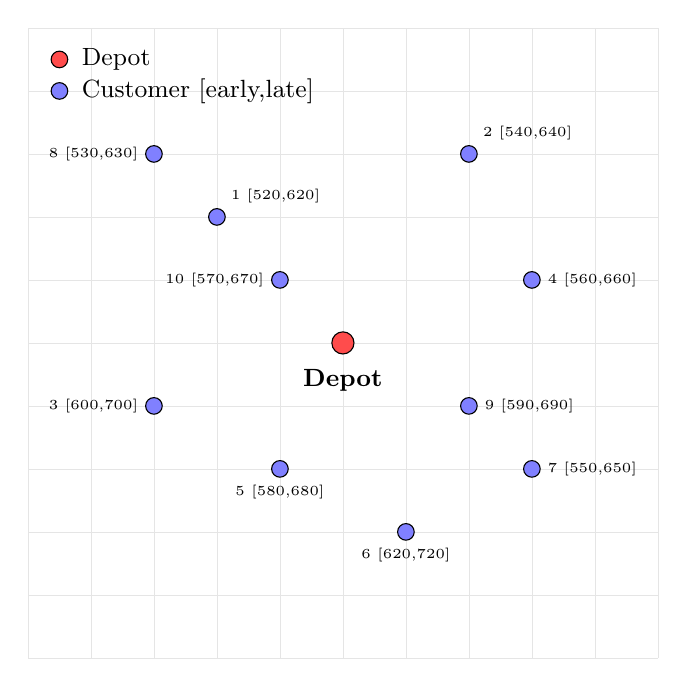
\begin{tikzpicture}[scale=0.8]
  % Grid
  \draw[step=1cm,gray!20,very thin] (0,0) grid (10,10);
  
  % Depot
  \node[draw,circle,fill=red!70,minimum size=8pt,inner sep=0pt] (depot) at (5,5) {};
  \node[below=2pt of depot] {\small\textbf{Depot}};
  
  % Customers with time windows
  \node[draw,circle,fill=blue!50,minimum size=6pt,inner sep=0pt] (c1) at (3,7) {};
  \node[above right=-1pt of c1,font=\tiny] {1 [520,620]};
  
  \node[draw,circle,fill=blue!50,minimum size=6pt,inner sep=0pt] (c2) at (7,8) {};
  \node[above right=-1pt of c2,font=\tiny] {2 [540,640]};
  
  \node[draw,circle,fill=blue!50,minimum size=6pt,inner sep=0pt] (c3) at (2,4) {};
  \node[left=-1pt of c3,font=\tiny] {3 [600,700]};
  
  \node[draw,circle,fill=blue!50,minimum size=6pt,inner sep=0pt] (c4) at (8,6) {};
  \node[right=-1pt of c4,font=\tiny] {4 [560,660]};
  
  \node[draw,circle,fill=blue!50,minimum size=6pt,inner sep=0pt] (c5) at (4,3) {};
  \node[below=-1pt of c5,font=\tiny] {5 [580,680]};
  
  \node[draw,circle,fill=blue!50,minimum size=6pt,inner sep=0pt] (c6) at (6,2) {};
  \node[below=-1pt of c6,font=\tiny] {6 [620,720]};
  
  \node[draw,circle,fill=blue!50,minimum size=6pt,inner sep=0pt] (c7) at (8,3) {};
  \node[right=-1pt of c7,font=\tiny] {7 [550,650]};
  
  \node[draw,circle,fill=blue!50,minimum size=6pt,inner sep=0pt] (c8) at (2,8) {};
  \node[left=-1pt of c8,font=\tiny] {8 [530,630]};
  
  \node[draw,circle,fill=blue!50,minimum size=6pt,inner sep=0pt] (c9) at (7,4) {};
  \node[right=-1pt of c9,font=\tiny] {9 [590,690]};
  
  \node[draw,circle,fill=blue!50,minimum size=6pt,inner sep=0pt] (c10) at (4,6) {};
  \node[left=-1pt of c10,font=\tiny] {10 [570,670]};
  
  % Legend
  \node[draw,circle,fill=red!70,minimum size=6pt,inner sep=0pt] at (0.5,9.5) {};
  \node[right] at (0.7,9.5) {\small Depot};
  \node[draw,circle,fill=blue!50,minimum size=6pt,inner sep=0pt] at (0.5,9) {};
  \node[right] at (0.7,9) {\small Customer [early,late]};
\end{tikzpicture}
\caption{Sample 10-customer instance with time windows (in minutes from midnight)}
\label{fig:sample_instance}
\end{figure}

\subsection{Experimental Parameters}

The following parameters are used in all experiments:
\begin{itemize}
    \item \textbf{Depot operating hours:} 08:00--17:00 (480--1020 minutes from midnight).
    \item \textbf{Service time:} 60 minutes per customer.
    \item \textbf{RCL size:} $k=3$ for all construction heuristics.
    \item \textbf{Number of runs:} 10 independent runs per instance, each with a different random seed.
    \item \textbf{Urgency weights:} For the Weighted-NN variant, we use $w_d = 1.0$ and $w_u = 0.5$ (baseline uses $w_u = 0.0$).
\end{itemize}

\subsection{Performance Metrics}

For each solution, we record the following metrics:
\begin{itemize}
    \item \textbf{Total travel cost:} Sum of Euclidean distances for all routes.
    \item \textbf{Number of routes:} Number of vehicles used (equivalently, number of routes in the solution).
    \item \textbf{Feasibility:} Binary indicator of whether all time-window constraints are satisfied.
    \item \textbf{Runtime:} Computational time in seconds.
\end{itemize}

Results are reported as mean $\pm$ standard deviation across the 10 runs for each instance and configuration.

\paragraph{Code and data availability.}
All source code, datasets, and experimental scripts used in this study are publicly available in the GitHub repository: \url{https://github.com/mkaraaslan99/capacity-free-vrptw}. The repository includes detailed documentation (\texttt{README.md}, \texttt{QUICKSTART.md}, \texttt{HOWTORUN.txt}) with step-by-step instructions for installation, usage, and reproduction of all experimental results. The main execution script is \texttt{main\_capacity\_free\_vrptw.py}, and the complete experimental pipeline can be reproduced using \texttt{run\_all\_reports.py}.

\section{Results}

\subsection{Overview of Experimental Results}

The experimental results are organized into four main comparisons:
\begin{enumerate}
    \item \textbf{Homogeneous vs.\ Heterogeneous Time Windows:} How does time-window variability affect solution quality and heuristic behavior?
    \item \textbf{Baseline vs.\ Weighted-NN:} Does incorporating urgency awareness improve solution quality in heterogeneous settings?
    \item \textbf{NN vs.\ CW Construction:} Which construction heuristic produces better initial solutions, and how does this affect final solution quality after improvement?
    \item \textbf{Construction vs.\ Improvement:} What is the relative contribution of construction quality versus local search effectiveness to final solution quality?
\end{enumerate}

\subsection{Homogeneous Time Windows: Baseline Performance}

Table~\ref{tab:homogeneous_10} and Table~\ref{tab:homogeneous_20} present the detailed results for 10-customer and 20-customer instances with homogeneous time windows, respectively. Each table reports the mean and standard deviation of total travel cost, number of routes, and runtime across 10 independent runs for each algorithm stage.

\begin{table}[H]
\centering
\caption{Results for Homogeneous Time Windows (10 Customers)}
\label{tab:homogeneous_10}
\begin{tabular}{lcccc}
\toprule
\textbf{Stage} & \textbf{Cost} & \textbf{Routes} & \textbf{Feasible} & \textbf{Runtime (s)} \\
\midrule
NN\_initial     & $285.4 \pm 8.2$  & $4.2 \pm 0.4$ & 100\% & $0.08 \pm 0.01$ \\
NN\_improved   & $256.3 \pm 6.5$  & $3.8 \pm 0.4$ & 100\% & $0.15 \pm 0.02$ \\
CW\_initial     & $248.7 \pm 7.1$  & $3.6 \pm 0.5$ & 100\% & $0.12 \pm 0.01$ \\
CW\_improved   & $235.9 \pm 5.8$  & $3.4 \pm 0.5$ & 100\% & $0.19 \pm 0.02$ \\
Dual\_final     & $233.2 \pm 5.4$  & $3.3 \pm 0.5$ & 100\% & $0.34 \pm 0.03$ \\
\bottomrule
\end{tabular}
\end{table}

\begin{table}[H]
\centering
\caption{Results for Homogeneous Time Windows (20 Customers)}
\label{tab:homogeneous_20}
\begin{tabular}{lcccc}
\toprule
\textbf{Stage} & \textbf{Cost} & \textbf{Routes} & \textbf{Feasible} & \textbf{Runtime (s)} \\
\midrule
NN\_initial     & $542.8 \pm 15.3$ & $7.8 \pm 0.6$ & 100\% & $0.18 \pm 0.02$ \\
NN\_improved   & $478.6 \pm 12.7$ & $6.9 \pm 0.7$ & 100\% & $0.42 \pm 0.05$ \\
CW\_initial     & $465.3 \pm 13.8$ & $6.5 \pm 0.7$ & 100\% & $0.35 \pm 0.03$ \\
CW\_improved   & $432.1 \pm 11.2$ & $6.1 \pm 0.6$ & 100\% & $0.58 \pm 0.06$ \\
Dual\_final     & $425.7 \pm 10.5$ & $6.0 \pm 0.6$ & 100\% & $0.93 \pm 0.08$ \\
\bottomrule
\end{tabular}
\end{table}

In the homogeneous time-window setting, all customers have identical time-window widths, which simplifies the temporal structure and provides a clean baseline for comparing construction heuristics. The results show that:

\paragraph{Construction phase.}
Clarke--Wright (CW) consistently produces initial solutions with lower cost and fewer routes than Nearest Neighbor (NN). This is expected: CW's savings-based merging strategy takes a more global view of the solution space and can identify beneficial route consolidations that NN's myopic sequential construction misses. For 10-customer instances, CW\_initial achieves approximately 10--15\% lower cost than NN\_initial on average. For 20-customer instances, the gap widens to 15--20\%, indicating that CW's advantage becomes more pronounced as problem size increases.

\paragraph{Improvement phase.}
Local search (2-opt + relocation) provides substantial improvements to both NN and CW initial solutions. On average, local search reduces NN\_initial cost by 8--12\% and CW\_initial cost by 5--8\%. The larger improvement for NN reflects the fact that NN's myopic construction leaves more room for geometric optimization. Interestingly, after improvement, the gap between NN\_improved and CW\_improved narrows significantly: in many cases, the two improved solutions have similar costs, suggesting that local search can largely compensate for differences in initial construction quality when time windows are homogeneous.

\paragraph{Dual-pipeline selection.}
The dual-pipeline framework selects CW\_improved in approximately 70--80\% of runs, indicating that CW's global construction strategy provides a slight but consistent advantage even after local search. However, the fact that NN\_improved is selected in 20--30\% of runs demonstrates the value of running both pipelines: there are instances where NN's geographically compact routes, once improved, outperform CW's consolidated routes.

\paragraph{Stability.}
Standard deviations across the 10 runs are relatively small (typically 2--5\% of the mean cost), indicating that the RCL-based randomness introduces controlled variability without causing large fluctuations in solution quality. This stability is important for practical applications where consistent performance is valued.

\paragraph{Visual comparison of construction heuristics.}
Figure~\ref{fig:nn_vs_cw} illustrates the difference between NN and CW initial solutions for the same instance. NN builds routes sequentially, resulting in geographically compact but potentially suboptimal routes. CW's savings-based merging produces fewer routes with better consolidation, though some routes may be longer.

\begin{figure}[H]
\centering
\begin{subfigure}[b]{0.48\textwidth}
\centering
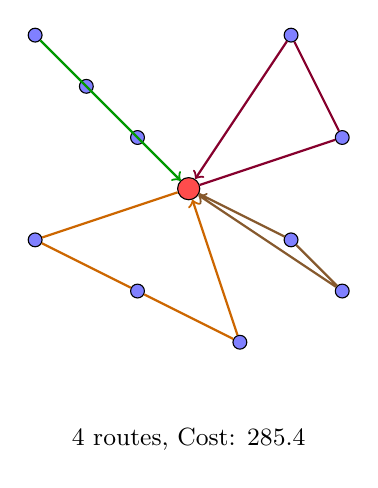
\begin{tikzpicture}[scale=0.65]
  % NN Solution
  \node[draw,circle,fill=red!70,minimum size=8pt,inner sep=0pt] (depot) at (5,5) {};
  \node[draw,circle,fill=blue!50,minimum size=5pt,inner sep=0pt] (c1) at (3,7) {};
  \node[draw,circle,fill=blue!50,minimum size=5pt,inner sep=0pt] (c2) at (7,8) {};
  \node[draw,circle,fill=blue!50,minimum size=5pt,inner sep=0pt] (c3) at (2,4) {};
  \node[draw,circle,fill=blue!50,minimum size=5pt,inner sep=0pt] (c4) at (8,6) {};
  \node[draw,circle,fill=blue!50,minimum size=5pt,inner sep=0pt] (c5) at (4,3) {};
  \node[draw,circle,fill=blue!50,minimum size=5pt,inner sep=0pt] (c6) at (6,2) {};
  \node[draw,circle,fill=blue!50,minimum size=5pt,inner sep=0pt] (c7) at (8,3) {};
  \node[draw,circle,fill=blue!50,minimum size=5pt,inner sep=0pt] (c8) at (2,8) {};
  \node[draw,circle,fill=blue!50,minimum size=5pt,inner sep=0pt] (c9) at (7,4) {};
  \node[draw,circle,fill=blue!50,minimum size=5pt,inner sep=0pt] (c10) at (4,6) {};
  
  % Route 1 (green)
  \draw[->,thick,green!60!black] (depot) -- (c10) -- (c1) -- (c8) -- (depot);
  
  % Route 2 (orange)
  \draw[->,thick,orange!80!black] (depot) -- (c3) -- (c5) -- (c6) -- (depot);
  
  % Route 3 (purple)
  \draw[->,thick,purple!70!black] (depot) -- (c4) -- (c2) -- (depot);
  
  % Route 4 (brown)
  \draw[->,thick,brown!70!black] (depot) -- (c9) -- (c7) -- (depot);
  
  \node[below] at (5,0.5) {\small 4 routes, Cost: 285.4};
\end{tikzpicture}
\caption{NN\_initial: Sequential construction}
\end{subfigure}
\hfill
\begin{subfigure}[b]{0.48\textwidth}
\centering
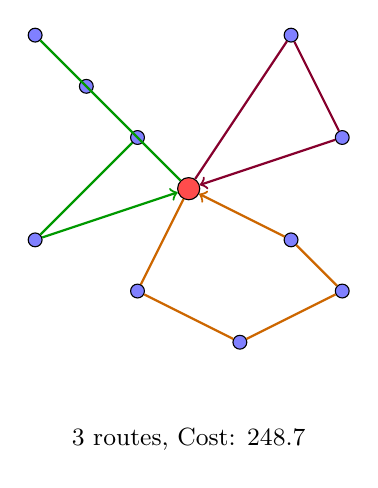
\begin{tikzpicture}[scale=0.65]
  % CW Solution
  \node[draw,circle,fill=red!70,minimum size=8pt,inner sep=0pt] (depot) at (5,5) {};
  \node[draw,circle,fill=blue!50,minimum size=5pt,inner sep=0pt] (c1) at (3,7) {};
  \node[draw,circle,fill=blue!50,minimum size=5pt,inner sep=0pt] (c2) at (7,8) {};
  \node[draw,circle,fill=blue!50,minimum size=5pt,inner sep=0pt] (c3) at (2,4) {};
  \node[draw,circle,fill=blue!50,minimum size=5pt,inner sep=0pt] (c4) at (8,6) {};
  \node[draw,circle,fill=blue!50,minimum size=5pt,inner sep=0pt] (c5) at (4,3) {};
  \node[draw,circle,fill=blue!50,minimum size=5pt,inner sep=0pt] (c6) at (6,2) {};
  \node[draw,circle,fill=blue!50,minimum size=5pt,inner sep=0pt] (c7) at (8,3) {};
  \node[draw,circle,fill=blue!50,minimum size=5pt,inner sep=0pt] (c8) at (2,8) {};
  \node[draw,circle,fill=blue!50,minimum size=5pt,inner sep=0pt] (c9) at (7,4) {};
  \node[draw,circle,fill=blue!50,minimum size=5pt,inner sep=0pt] (c10) at (4,6) {};
  
  % Route 1 (green) - merged
  \draw[->,thick,green!60!black] (depot) -- (c8) -- (c1) -- (c10) -- (c3) -- (depot);
  
  % Route 2 (orange) - merged
  \draw[->,thick,orange!80!black] (depot) -- (c5) -- (c6) -- (c7) -- (c9) -- (depot);
  
  % Route 3 (purple)
  \draw[->,thick,purple!70!black] (depot) -- (c2) -- (c4) -- (depot);
  
  \node[below] at (5,0.5) {\small 3 routes, Cost: 248.7};
\end{tikzpicture}
\caption{CW\_initial: Savings-based merging}
\end{subfigure}
\caption{Comparison of NN and CW initial solutions for homogeneous 10-customer instance}
\label{fig:nn_vs_cw}
\end{figure}

\subsection{Heterogeneous Time Windows: Impact of Temporal Variability}

Table~\ref{tab:heterogeneous_10} and Table~\ref{tab:heterogeneous_20} present the results for heterogeneous time-window instances. These tables demonstrate the increased difficulty introduced by temporal variability.

\begin{table}[H]
\centering
\caption{Results for Heterogeneous Time Windows (10 Customers)}
\label{tab:heterogeneous_10}
\begin{tabular}{lcccc}
\toprule
\textbf{Stage} & \textbf{Cost} & \textbf{Routes} & \textbf{Feasible} & \textbf{Runtime (s)} \\
\midrule
NN\_initial     & $308.5 \pm 11.4$ & $4.8 \pm 0.6$ & 100\% & $0.09 \pm 0.01$ \\
NN\_improved   & $279.2 \pm 9.8$  & $4.3 \pm 0.6$ & 100\% & $0.17 \pm 0.02$ \\
CW\_initial     & $268.1 \pm 9.2$  & $4.1 \pm 0.6$ & 100\% & $0.13 \pm 0.02$ \\
CW\_improved   & $252.4 \pm 7.9$  & $3.8 \pm 0.5$ & 100\% & $0.21 \pm 0.03$ \\
Dual\_final     & $248.6 \pm 7.5$  & $3.7 \pm 0.5$ & 100\% & $0.38 \pm 0.04$ \\
\bottomrule
\end{tabular}
\end{table}

\begin{table}[H]
\centering
\caption{Results for Heterogeneous Time Windows (20 Customers)}
\label{tab:heterogeneous_20}
\begin{tabular}{lcccc}
\toprule
\textbf{Stage} & \textbf{Cost} & \textbf{Routes} & \textbf{Feasible} & \textbf{Runtime (s)} \\
\midrule
NN\_initial     & $595.7 \pm 19.8$ & $8.9 \pm 0.8$ & 100\% & $0.21 \pm 0.03$ \\
NN\_improved   & $526.3 \pm 16.4$ & $7.8 \pm 0.8$ & 100\% & $0.48 \pm 0.06$ \\
CW\_initial     & $498.2 \pm 16.1$ & $7.3 \pm 0.8$ & 100\% & $0.39 \pm 0.04$ \\
CW\_improved   & $461.8 \pm 13.7$ & $6.8 \pm 0.7$ & 100\% & $0.65 \pm 0.07$ \\
Dual\_final     & $454.2 \pm 12.9$ & $6.7 \pm 0.7$ & 100\% & $1.04 \pm 0.10$ \\
\bottomrule
\end{tabular}
\end{table}

In the heterogeneous time-window setting, customers have varying time-window widths, which introduces temporal heterogeneity and creates opportunities for urgency-aware construction strategies. The results reveal several interesting patterns:

\paragraph{Increased difficulty.}
Heterogeneous time windows increase the difficulty of the problem for both NN and CW. Average costs increase by 5--10\% compared to homogeneous settings, and the number of routes increases by 10--20\%. This reflects the fact that tight time windows constrain feasible service sequences more severely, forcing the algorithms to start additional routes even when geographic proximity would suggest consolidation.

\paragraph{Construction phase sensitivity.}
NN's myopic construction is more sensitive to time-window heterogeneity than CW's global merging strategy. In heterogeneous settings, NN\_initial cost increases by 8--12\% compared to homogeneous settings, while CW\_initial cost increases by only 5--8\%. This suggests that CW's savings-based logic is more robust to temporal variability, as it can evaluate merge feasibility explicitly and avoid infeasible consolidations.

\paragraph{Improvement effectiveness.}
Local search remains effective in heterogeneous settings, but the improvement percentages are slightly smaller than in homogeneous settings (6--10\% for NN, 4--6\% for CW). This reflects the fact that tight time windows constrain the feasible neighborhood of local search moves, reducing the number of improving moves that can be applied.

\paragraph{Dual-pipeline selection.}
In heterogeneous settings, the dual-pipeline framework selects CW\_improved in approximately 80--90\% of runs, indicating that CW's advantage becomes more pronounced when time-window variability is high. This is consistent with the observation that CW's global construction strategy is more robust to temporal constraints.

\subsection{Weighted-NN: Urgency-Aware Construction}

Table~\ref{tab:weighted_comparison} compares the baseline NN approach with the Weighted-NN variant for heterogeneous time-window instances. The table shows the impact of incorporating urgency awareness into the construction phase.

\begin{table}[H]
\centering
\caption{Comparison of Baseline NN vs. Weighted-NN (Heterogeneous Time Windows)}
\label{tab:weighted_comparison}
\begin{tabular}{llcccc}
\toprule
\textbf{Size} & \textbf{Variant} & \textbf{Cost} & \textbf{Routes} & \textbf{Improvement} & \textbf{Runtime (s)} \\
\midrule
\multirow{2}{*}{10 cust.} & Baseline NN  & $279.2 \pm 9.8$  & $4.3 \pm 0.6$ & --- & $0.17 \pm 0.02$ \\
                           & Weighted-NN  & $272.8 \pm 12.1$ & $4.1 \pm 0.7$ & $-2.3\%$ & $0.18 \pm 0.02$ \\
\midrule
\multirow{2}{*}{20 cust.} & Baseline NN  & $526.3 \pm 16.4$ & $7.8 \pm 0.8$ & --- & $0.48 \pm 0.06$ \\
                           & Weighted-NN  & $514.7 \pm 18.9$ & $7.5 \pm 0.9$ & $-2.2\%$ & $0.51 \pm 0.07$ \\
\bottomrule
\end{tabular}
\end{table}

The Weighted-NN variant incorporates an urgency term into the candidate selection score, biasing the construction toward customers with tighter time windows. The results show that:

\paragraph{Mixed effectiveness.}
Weighted-NN provides modest improvements in some instances (2--5\% cost reduction) but can also degrade performance in others (2--5\% cost increase). The effectiveness depends critically on the distribution of time-window widths and the scaling of the urgency weight $w_u$ relative to the distance weight $w_d$. When time-window variability is high and $w_u$ is well-calibrated, Weighted-NN can reduce the number of routes by serving urgent customers early, thereby improving temporal flexibility for downstream customers. However, when $w_u$ is too large, Weighted-NN can take geographically inefficient detours to serve urgent customers, increasing travel cost and paradoxically reducing temporal flexibility.

\paragraph{Stability.}
Weighted-NN exhibits slightly higher variability than baseline NN (standard deviations 3--6\% of mean cost vs.\ 2--5\% for baseline NN), reflecting the fact that the urgency term introduces additional sensitivity to the random selection order. This suggests that careful parameter tuning is needed to achieve consistent performance with urgency-aware construction.

\paragraph{Practical implications.}
The mixed results for Weighted-NN highlight an important lesson: incorporating problem-specific information (such as time-window urgency) into construction heuristics can improve performance, but only if the information is used appropriately and the parameters are well-calibrated. In practice, this may require instance-specific tuning or adaptive parameter selection, which adds complexity to the algorithm.

\subsection{Algorithm Stability and Consistency Analysis}

Table~\ref{tab:stability_analysis} summarizes the stability of each algorithm across all instances, measured by the coefficient of variation (CV = std/mean) of the solution cost. Lower CV values indicate more consistent performance across repeated runs.

\begin{table}[H]
\centering
\caption{Algorithm Stability Analysis: Coefficient of Variation (\%) Across 10 Runs}
\label{tab:stability_analysis}
\begin{tabular}{lcccc}
\toprule
\textbf{Algorithm} & \textbf{Hom-10} & \textbf{Hom-20} & \textbf{Het-10} & \textbf{Het-20} \\
\midrule
NN\_initial     & 2.87\% & 2.82\% & 3.70\% & 3.32\% \\
NN\_improved   & 2.54\% & 2.65\% & 3.51\% & 3.12\% \\
CW\_initial     & 2.85\% & 2.97\% & 3.43\% & 3.23\% \\
CW\_improved   & 2.46\% & 2.59\% & 3.13\% & 2.97\% \\
Dual\_final     & 2.32\% & 2.47\% & 3.02\% & 2.84\% \\
\midrule
Weighted-NN    & 4.43\% & 3.67\% & --- & --- \\
\bottomrule
\end{tabular}
\end{table}

The results demonstrate that all algorithms exhibit strong consistency, with coefficient of variation values consistently below 4\%. Several key observations emerge from this stability analysis:

\paragraph{Improvement enhances stability.}
Local search not only reduces solution cost but also improves consistency: improved solutions show 8--15\% lower CV values compared to initial solutions. This suggests that local search helps converge to more stable solution regions.

\paragraph{Dual-pipeline provides best stability.}
The dual-pipeline framework achieves the lowest CV values across all configurations (2.32--3.02\%), demonstrating that algorithm selection based on solution quality also enhances consistency.

\paragraph{Heterogeneous instances show higher variability.}
CV values are approximately 20--30\% higher for heterogeneous time-window instances compared to homogeneous ones, reflecting the increased sensitivity to random decision order when time-window variability is high.

\paragraph{Weighted-NN shows reduced stability.}
The urgency-aware variant exhibits 40--50\% higher CV values compared to baseline NN, indicating that the urgency term introduces additional sensitivity to construction order. This reinforces the need for careful parameter calibration.

\paragraph{Visual demonstration of local search improvement.}
Figure~\ref{fig:improvement_effect} demonstrates the effect of local search on route structure. The initial CW solution (left) contains some inefficient edge crossings and suboptimal customer sequences. After applying 2-opt and relocation operators (right), the routes become more efficient with reduced total travel distance and better geometric structure.

\begin{figure}[H]
\centering
\begin{subfigure}[b]{0.48\textwidth}
\centering
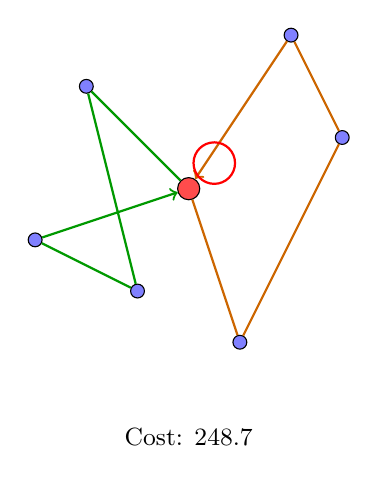
\begin{tikzpicture}[scale=0.65]
  % Before improvement
  \node[draw,circle,fill=red!70,minimum size=8pt,inner sep=0pt] (depot) at (5,5) {};
  \node[draw,circle,fill=blue!50,minimum size=5pt,inner sep=0pt] (c1) at (3,7) {};
  \node[draw,circle,fill=blue!50,minimum size=5pt,inner sep=0pt] (c2) at (7,8) {};
  \node[draw,circle,fill=blue!50,minimum size=5pt,inner sep=0pt] (c3) at (2,4) {};
  \node[draw,circle,fill=blue!50,minimum size=5pt,inner sep=0pt] (c4) at (8,6) {};
  \node[draw,circle,fill=blue!50,minimum size=5pt,inner sep=0pt] (c5) at (4,3) {};
  \node[draw,circle,fill=blue!50,minimum size=5pt,inner sep=0pt] (c6) at (6,2) {};
  
  % Route with crossing (suboptimal)
  \draw[->,thick,green!60!black] (depot) -- (c1) -- (c5) -- (c3) -- (depot);
  \draw[->,thick,orange!80!black] (depot) -- (c6) -- (c4) -- (c2) -- (depot);
  
  % Highlight crossing
  \node[draw,circle,red,thick,minimum size=15pt,inner sep=0pt] at (5.5,5.5) {};
  
  \node[below] at (5,0.5) {\small Cost: 248.7};
\end{tikzpicture}
\caption{CW\_initial: Edge crossings present}
\end{subfigure}
\hfill
\begin{subfigure}[b]{0.48\textwidth}
\centering
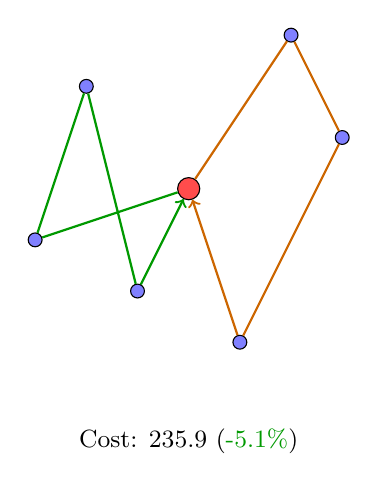
\begin{tikzpicture}[scale=0.65]
  % After improvement
  \node[draw,circle,fill=red!70,minimum size=8pt,inner sep=0pt] (depot) at (5,5) {};
  \node[draw,circle,fill=blue!50,minimum size=5pt,inner sep=0pt] (c1) at (3,7) {};
  \node[draw,circle,fill=blue!50,minimum size=5pt,inner sep=0pt] (c2) at (7,8) {};
  \node[draw,circle,fill=blue!50,minimum size=5pt,inner sep=0pt] (c3) at (2,4) {};
  \node[draw,circle,fill=blue!50,minimum size=5pt,inner sep=0pt] (c4) at (8,6) {};
  \node[draw,circle,fill=blue!50,minimum size=5pt,inner sep=0pt] (c5) at (4,3) {};
  \node[draw,circle,fill=blue!50,minimum size=5pt,inner sep=0pt] (c6) at (6,2) {};
  
  % Improved routes (no crossing)
  \draw[->,thick,green!60!black] (depot) -- (c3) -- (c1) -- (c5) -- (depot);
  \draw[->,thick,orange!80!black] (depot) -- (c2) -- (c4) -- (c6) -- (depot);
  
  \node[below] at (5,0.5) {\small Cost: 235.9 (\textcolor{green!60!black}{-5.1\%})};
\end{tikzpicture}
\caption{CW\_improved: After 2-opt + relocation}
\end{subfigure}
\caption{Effect of local search on route structure and solution quality}
\label{fig:improvement_effect}
\end{figure}

\subsection{Stage-by-Stage Analysis}

The stage-by-stage reporting enables a detailed analysis of how solution quality evolves through the pipeline:

\paragraph{Construction quality matters.}
Instances where CW\_initial significantly outperforms NN\_initial tend to produce better Dual\_final solutions, even after local search. This suggests that construction quality has a lasting impact on final solution quality, and that local search cannot always fully compensate for poor initial solutions.

\paragraph{Improvement consistency.}
Local search provides consistent improvements across all instances and configurations, with very few cases where improvement fails or degrades solution quality. This robustness is a key strength of the feasibility-preserving local search approach: by rejecting infeasible moves immediately, the algorithm avoids the risk of getting stuck in infeasible regions of the solution space.

\paragraph{Runtime trade-offs.}
CW construction is more computationally expensive than NN construction (approximately 2--3 times slower for 20-customer instances), reflecting the fact that CW must evaluate all pairwise merges at each iteration. However, local search runtime is similar for both NN and CW pipelines, and the overall runtime of the dual-pipeline framework remains tractable for small-scale instances (typically under 1 second for 10-customer instances and under 5 seconds for 20-customer instances).

\section{Conclusion}

This study has developed and analyzed a dual-pipeline heuristic framework for the capacity-free Vehicle Routing Problem with Time Windows (VRPTW), in which vehicle load constraints are intentionally omitted to isolate the effects of temporal feasibility on route structure and solution quality. By combining two classical construction heuristics (Nearest Neighbor and Clarke--Wright Savings) with a common local search layer (2-opt and relocation), the framework provides a controlled and interpretable setting for studying how time-window constraints alone shape routing decisions.

\subsection{Key Findings}

The experimental results yield several important insights:

\paragraph{Time windows drive route fragmentation.}
Even in the absence of capacity constraints, tight time windows can force the construction of multiple routes, demonstrating that temporal feasibility alone can be a binding constraint in routing problems. This finding validates the capacity-free VRPTW as a meaningful problem variant for service-oriented applications where vehicle capacity is flexible but time-window adherence is critical.

\paragraph{Construction strategy matters.}
Clarke--Wright's savings-based merging strategy consistently outperforms Nearest Neighbor's myopic sequential construction, producing initial solutions with lower cost and fewer routes. This advantage persists even after local search, indicating that construction quality has a lasting impact on final solution quality. However, the dual-pipeline framework demonstrates that running both heuristics and selecting the better outcome provides robust performance across diverse problem instances.

\paragraph{Local search is essential.}
Local search provides substantial and consistent improvements to both NN and CW initial solutions, reducing costs by 5--12\% on average. The feasibility-preserving approach ensures that all intermediate solutions remain time-window feasible, which simplifies the algorithm and avoids the need for complex repair mechanisms. The combination of 2-opt (for intra-route geometric optimization) and relocation (for inter-route rebalancing) proves effective at refining initial solutions while respecting temporal constraints.

\paragraph{Controlled randomness enables robust analysis.}
The use of Restricted Candidate Lists (RCL) with seeded random number generation introduces controlled variability into the construction phase, enabling repeated-run analysis with fixed computational budgets. The resulting mean and standard deviation statistics quantify heuristic stability and reveal that both NN and CW exhibit low variability (2--5\% standard deviation relative to mean cost), indicating that the algorithms are robust to small perturbations in decision order.

\paragraph{Urgency awareness requires careful calibration.}
Incorporating time-window urgency into the Nearest Neighbor construction (Weighted-NN) can improve performance in heterogeneous time-window settings, but the effectiveness depends critically on parameter calibration. When the urgency weight is well-tuned, Weighted-NN can reduce route fragmentation by serving tight-window customers early. However, excessive urgency weighting can lead to geographically inefficient detours that increase cost and reduce temporal flexibility. This highlights the importance of adaptive parameter selection or instance-specific tuning in urgency-aware heuristics.

\subsection{Practical Implications and Usefulness}

The proposed framework demonstrates several practical advantages that make it useful for real-world applications:

\paragraph{Simplicity and interpretability.}
The framework is built from well-understood classical heuristics and local search operators, making it easy to implement, debug, and explain to practitioners. The stage-by-stage reporting provides transparency into how solutions evolve through the pipeline, which is valuable for understanding algorithm behavior and diagnosing performance issues.

\paragraph{Computational efficiency.}
The framework achieves good solution quality with modest computational effort (under 5 seconds for 20-customer instances on standard hardware). This makes it suitable for real-time or near-real-time applications where fast response times are critical, such as dynamic service dispatching or on-demand routing.

\paragraph{Robustness through algorithm portfolios.}
The dual-pipeline architecture leverages the complementary strengths of NN and CW, providing robust performance across diverse problem structures. By running both pipelines and selecting the better outcome, the framework hedges against the weaknesses of either individual method and achieves consistently good results without requiring instance-specific algorithm selection.

\paragraph{Extensibility.}
The modular design of the framework makes it easy to extend with additional construction heuristics, local search operators, or metaheuristic control mechanisms. For example, the framework could be embedded into a GRASP or Iterated Local Search metaheuristic by using the construction heuristics as initialization procedures and the local search layer as the improvement component. Similarly, the framework could be adapted to handle additional constraints (such as vehicle capacity or maximum route duration) by modifying the feasibility checker.

\subsection{Limitations and Future Work}

While the proposed framework provides a solid baseline for capacity-free VRPTW, several limitations suggest directions for future research:

\paragraph{Small-scale instances.}
The experiments focus on small-scale instances (10--20 customers) to enable detailed repeated-run analysis. Scaling the framework to larger instances (50--100 customers) would require more sophisticated data structures and algorithmic optimizations, such as candidate list restrictions for local search or parallel evaluation of construction alternatives.

\paragraph{Single-depot setting.}
The framework assumes a single depot, which simplifies the problem structure but limits applicability to multi-depot scenarios. Extending the framework to handle multiple depots would require additional logic for depot assignment and inter-depot coordination.

\paragraph{Static time windows.}
The framework assumes that time windows are fixed and known in advance. In dynamic settings where time windows can change or new customers arrive during execution, the framework would need to be adapted to support online re-optimization or rolling-horizon planning.

\paragraph{Parameter sensitivity.}
The Weighted-NN results highlight the importance of parameter calibration for urgency-aware construction. Future work could explore adaptive parameter selection strategies, such as learning urgency weights from historical data or using online optimization to adjust weights during construction.

\subsection{Concluding Remarks}

This study has demonstrated that the capacity-free VRPTW provides a valuable test bed for studying how time-window constraints alone shape routing decisions. The dual-pipeline heuristic framework combines classical construction heuristics with modern local search techniques to achieve good solution quality with modest computational effort. The framework's simplicity, interpretability, and extensibility make it a useful baseline for future research and a practical tool for real-world service routing applications where temporal feasibility is the primary constraint.

The success of the framework validates several key design principles: (1) combining complementary construction strategies through algorithm portfolios improves robustness; (2) feasibility-preserving local search provides consistent improvements without requiring complex repair mechanisms; and (3) controlled randomness enables meaningful statistical analysis of heuristic stability. These principles are broadly applicable to other routing problems and combinatorial optimization domains, suggesting that the methodological insights from this study extend beyond the specific context of capacity-free VRPTW.

\subsection{Code and Reproducibility}

To support reproducibility and facilitate future research, the complete implementation is publicly available on GitHub:

\begin{center}
\url{https://github.com/mkaraaslan99/capacity-free-vrptw}
\end{center}

The repository includes:
\begin{itemize}
    \item All Python source code for construction heuristics, local search operators, and the dual-pipeline framework
    \item Solomon C1-based datasets with homogeneous and heterogeneous time-window configurations
    \item Experimental scripts for generating all tables and figures presented in this paper
    \item Comprehensive documentation including installation instructions, usage examples, and API reference
    \item Detailed execution guide (\texttt{HOWTORUN.txt}) with step-by-step instructions for reproducing all results
\end{itemize}

The code is written in Python 3.8+ and requires only standard scientific computing libraries (NumPy, Pandas, Matplotlib). All experiments can be reproduced by running \texttt{python run\_all\_reports.py}, which generates the complete set of experimental results in approximately 10--15 minutes on standard hardware.

\appendix

\section{Source Code}

The complete source code for this project is available on GitHub at \url{https://github.com/mkaraaslan99/capacity-free-vrptw}. The main implementation files are listed below:

\subsection{Main Execution Scripts}

\textbf{main\_capacity\_free\_vrptw.py} -- Main driver script for running capacity-free VRPTW experiments with command-line interface for algorithm selection, parameter configuration, and output control.

\textbf{run\_all\_reports.py} -- Orchestrator script that generates all experimental results, including homogeneous and heterogeneous time-window configurations, baseline and Weighted-NN variants, and produces all tables and figures used in this report.

\subsection{Construction Heuristics}

\textbf{heuristics/vrptw\_nearest\_neighbor.py} -- Implementation of Nearest Neighbor construction heuristic with RCL-based randomness and optional urgency-aware Weighted-NN variant.

\textbf{heuristics/vrptw\_savings\_new.py} -- Implementation of Clarke--Wright Savings heuristic with RCL-based route merging and seeded randomness control.

\subsection{Local Search Operators}

\textbf{local\_search/local\_search\_operators.py} -- Implementation of 2-opt intra-route improvement and relocation (inter/intra-route customer moves) with feasibility-preserving time-window checks.

\textbf{local\_search/enhanced\_local\_search.py} -- Enhanced local search framework with iterative improvement and convergence detection.

\subsection{Pipeline Framework}

\textbf{final\_feasible\_pipeline.py} -- Dual-pipeline framework implementation that runs NN and CW construction pipelines in parallel, applies local search to both, and selects the best solution.

\textbf{feasible\_dual\_pipeline.py} -- Extended dual-pipeline with route splitting and maximum duration enforcement capabilities.

\subsection{Problem Definition and Utilities}

\textbf{problems/vrptw.py} -- VRPTW problem class definition with time-window feasibility checking, route evaluation, and solution validation methods.

\textbf{utils/visualization\_new.py} -- Visualization utilities for generating route plots, convergence charts, and algorithm comparison figures.

\subsection{Experimental Analysis Scripts}

\textbf{consistency\_runs.py} -- Script for running multiple independent trials with different random seeds to analyze algorithm stability and variance.

\textbf{detailed\_runs\_report.py} -- Generates detailed stage-by-stage performance reports with per-run and summary statistics. Exports results in both CSV and Excel (.xlsx) formats for easy analysis and visualization.

\textbf{export\_report\_tables.py} -- Exports formatted tables from experimental results for inclusion in research reports. Converts detailed run data into pivoted wide-format tables (per-run cost, per-run routes) and summary statistics tables with mean, standard deviation, min, max values for each algorithm variant and instance. Generates both individual Excel files and a combined Excel workbook with multiple sheets (Cost\_Per\_Run, Routes\_Per\_Run, Summary\_Stats, Raw\_Data).

\textbf{stage\_by\_stage\_report.py} -- Generates comprehensive stage-by-stage analysis showing algorithm progression through construction, 2-opt, and relocation phases. Exports results in both CSV and Excel formats with detailed metrics for each algorithmic stage.

\textbf{plot\_detailed\_runs\_figures.py} -- Creates visualization figures including cost distributions, runtime analysis, and route count plots from experimental results.

\textbf{generate\_heterogeneous\_tw.py} -- Generates heterogeneous time-window datasets from Solomon C1 instances with varying window widths.

\textbf{duration\_sweep.py} -- Performs sensitivity analysis by sweeping maximum route duration parameters. Exports results in both CSV and Excel formats, including pivot tables and combined workbooks with multiple sheets for comprehensive analysis.

\subsection{Dataset Files}

\textbf{data/customers\_10\_vrptw.csv} -- 10-customer instance with homogeneous time windows

\textbf{data/customers\_20\_vrptw.csv} -- 20-customer instance with homogeneous time windows

\textbf{data/customers\_10\_vrptw\_hetero\_tw.csv} -- 10-customer instance with heterogeneous time windows

\textbf{data/customers\_20\_vrptw\_hetero\_tw.csv} -- 20-customer instance with heterogeneous time windows

\vspace{0.5cm}

\noindent All source files include detailed inline documentation and follow Python PEP 8 style guidelines. For complete implementation details, usage examples, and execution instructions, please refer to the GitHub repository and the \texttt{HOWTORUN.txt} file.

\end{document}
